% $Header: /cvsroot/latex-beamer/latex-beamer/solutions/generic-talks/generic-ornate-15min-45min.en.tex,v 1.5 2007/01/28 20:48:23 tantau Exp $

\documentclass[fleqn]{beamer}

% This file is a solution template for:

% - Giving a talk on some subject.
% - The talk is between 15min and 45min long.
% - Style is ornate.
 


% Copyright 2004 by Till Tantau <tantau@users.sourceforge.net>.
%
% In principle, this file can be redistributed and/or modified under
% the terms of the GNU Public License, version 2.
%
% However, this file is supposed to be a template to be modified
% for your own needs. For this reason, if you use this file as a
% template and not specifically distribute it as part of a another
% package/program, I grant the extra permission to freely copy and
% modify this file as you see fit and even to delete this copyright
% notice. 


\mode<presentation>
% {
%   \usetheme{Warsaw}
%   % or ...

%   \setbeamercovered{transparent}
%   % or whatever (possibly just delete it)
% }

\usepackage{beamerthemeshadow}
\usepackage[english,czech]{babel}
\usepackage{bibentry}
%\usepackage{natbib}
%\selectbiblanguage{czech}
\usepackage{url}
\usepackage{hyperref}
\usepackage{lmodern}
\def\uv#1{\glqq#1\grqq}
\usepackage{graphicx}
%\usepackage{listings}
% or whatever
\usepackage{amsmath}
\usepackage{xspace}
\usepackage{natbib}
\usepackage{float}
%\usepackage{wrapfig}
%\usepackage{sidecap}
%\usepackage{txfonts}            
\usepackage{color}
\usepackage{verbatim}
\usepackage{listings}


\usepackage[utf8]{inputenc}
% or whatever

%\usepackage{times}
\usepackage[T1]{fontenc}
% Or whatever. Note that the encoding and the font should match. If T1
% does not look nice, try deleting the line with the fontenc.


\title[VO \& Data Mining] % (optional, use only with long paper titles)
{Astar's  guide into astroinformatics concepts} 

\subtitle{... or what I wish to knew when I was younger} % (optional)

\author[Jaroslav Vážný] % (optional, use only with lots of authors)
{Jaroslav Vážný }
% - Use the \inst{?} command only if the authors have different
%   affiliation.

\institute[Universities of Somewhere and Elsewhere] % (optional, but mostly needed)
{

    Masarykova univerzita

}
% - Use the \inst command only if there are several affiliations.
% - Keep it simple, no one is interested in your street address.

%\date[Short Occasion] % (optional)
%{Date / Occasion}

\subject{Talks}
% This is only inserted into the PDF information catalog. Can be left
% out. 



% If you have a file called "university-logo-filename.xxx", where xxx
% is a graphic format that can be processed by latex or pdflatex,
% resp., then you can add a logo as follows:

\pgfdeclareimage[height=0.5cm]{university-logo}{sci-logo}
\logo{\pgfuseimage{university-logo}}



% Delete this, if you do not want the table of contents to pop up at
% the beginning of each subsection:
\AtBeginSubsection[]
{
  \begin{frame}<beamer>{Outline}
    \tableofcontents[currentsection,currentsubsection]
  \end{frame}
}


% If you wish to uncover everything in a step-wise fashion, uncomment
% the following command: 

%\beamerdefaultoverlayspecification{<+->}


\begin{document}
% vylepseny listing z http://texnik.de/TeXnik/listings/listing0.pdf
 \definecolor{hellgelb}{rgb}{1,1,0.8}
 \definecolor{colKeys}{rgb}{0,0,1}
 \definecolor{colIdentifier}{rgb}{0,0,0}
 \definecolor{colComments}{rgb}{1,0,0}
 \definecolor{colString}{rgb}{0,0.5,0}
 \lstset{%
   language={SQL},%
    morekeywords={In,AND,ASC,avg,CHECK,COMMIT,count,DECODE,DESC,DISTINCT,%
                 GROUP,IN,LIKE,NUMBER,ROLLBACK,SUBSTR,sum,VARCHAR2}%
 }

 \lstset{%
     float=hbp,%
     basicstyle=\ttfamily\small, %
%     identifierstyle=\color{colIdentifier}, %
%     keywordstyle=\color{colKeys}, %
     stringstyle=\color{colString}, %
     commentstyle=\color{colComments}, %
     columns=flexible, %
     tabsize=4, %
     frame=single, %
     extendedchars=true, %
     showspaces=false, %
     showstringspaces=false, %
   numbers=left, %
   numberstyle=\tiny, %
   breaklines=true, %
   backgroundcolor=\color{hellgelb}, %
   breakautoindent=true, %
   captionpos=b%
 }

 

%\begin{frame}
%  \begin{center}
%    \frametitle{Vítejte ...}
%    \small{Anybody who is not shocked by this subject has failed to understand it.}\cite{skala2005ukm} 
%  \end{center}
%\end{frame}



\begin{frame}
  \titlepage
\end{frame}


%\begin{frame}
%  \tableofcontents
%\end{frame}


\begin{frame}\frametitle{Abstract}
\small{Today's science lives in the virtual digitalized world. If we
  want to exploit the full potential of available data We have to be
  able to bump and grind in this world with ease and confidence.
  Computer science and technology in general are opportunities but
  require deep knowledge of the field.  This is a problem because
  unlike mathematics computer science is not standard part of the
  scientific curriculum (at least not now in the Czech Republic). This
  presentation is meant to be short introduction in the important
  concepts in computer science.  This is My personal point of view and
  it possible (and I hope) that other people see things in absolutely
  different light. What is my motivation? I have seen many brilliant
  physicists to struggle with simple tasks related with computers. I
  want to give young people some advices so they can deal with this
  subject with less pain.}



\end{frame}


\begin{frame}\frametitle{Motivation}
  There are two extreme cases one can see role of computers in science
  \begin{itemize}
  \item \textbf{Old school} Computer is just a tool. I want to focus
    on my science problem. I don't care what XML is.
  \item \textbf{Hackers} I want to know more ...;-) 

\bigskip

The best technique to avoid the troubles with computers is to have deep
knowledge about wide concepts in computer science. Paradoxically both
cases leads to the same conclusion!
  \end{itemize}
\end{frame}

\begin{section}{Overview}
\begin{frame}\frametitle{Concepts introduced in this talk}
  \begin{center}
    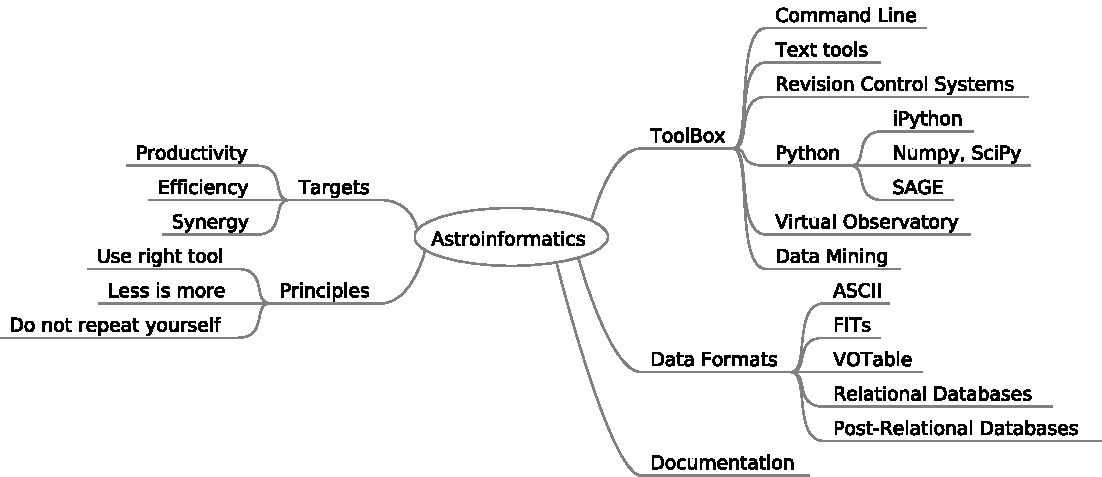
\includegraphics[width=1.0\textwidth]{overview}    
  \end{center}
\end{frame}
\end{section}



% ToolBox

\begin{section}{ToolBox}
  \begin{frame}\frametitle{Command Line}
  \begin{itemize}
    \item{Why is it important?}
    \begin{itemize}
      \item{Efficient dialog computer $\Longleftrightarrow$ human}
      \item{In all advanced tools (Programming, mathematica, CAD, \ldots)}
      \item{Cooperation, reusability, automatization }
    \end{itemize}

    \item{Where I can learn it?}
    \begin{itemize}
      \item MUNI: PV004, F4270, PV065 
      \item PEEPCODE: Meet the Command Line, Advanced Command Line  
    \end{itemize}
  \end{itemize}

%\begin{quotation} %this creates the heading for the dedication page
%{"What is it that makes us human? It's not something you "} 

%% \flushright{Marcus Wright}

%\end{quotation}


  \end{frame}

  \begin{frame}\frametitle{Examples}
  \begin{itemize}
    \item TAB 
    \item !! Repeat last command
    \item !\$ Repeat last agrument
    \item history command history
    \item CTRL+R search in history
  \end{itemize}
  \end{frame}

  
  \begin{frame}\frametitle{Text tools}
  \begin{itemize}
    \item{Why is it important?}
      \begin{itemize}
      \item "Everything" is a text
      \item head, tail, sed, awk, join, paste, vim, emacs \ldots
      \end{itemize}
 \item{Where I can learn it?}
  \begin{itemize}
      \item PEEPCODE: Meet Emacs, Smash Into Vim, Vim Emacs tutorials !!! 
  \end{itemize}
  \end{itemize}
  \end{frame}

\begin{frame}\frametitle{Examples}
  \begin{itemize}
    \item echo "AlDeBaraN" | tr "[:upper:]" "[:lower:]"
    \item vimdiff file1 file2
  \end{itemize}
  \end{frame}


  \begin{frame}\frametitle{Revison Control Systems}
  \begin{itemize}
    \item{Why is it important?}
      \begin{itemize}
      \item Content history
      \item Non-Linear Development
      \item Cooperation
      \end{itemize}
    \item{Where I can learn it?}
    \item PEEPCODE: Git, Mercurial
  \end{itemize}
  \end{frame}
\end{section}

\begin{frame}\frametitle{Examples}
      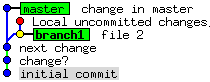
\includegraphics[scale = .5]{git1}    
      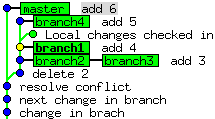
\includegraphics[scale = .5]{git2}    
%      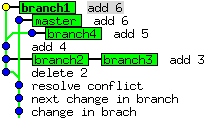
\includegraphics[scale = .5]{git3}    
      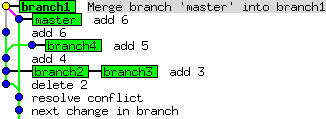
\includegraphics[scale = .5]{git4}    
\end{frame}


% Data formats

\begin{section}{Data Formats}
  %% \begin{frame}\frametitle{ASCII}
  %% \begin{itemize}
  %%   \item{Why is it important?}
  %%   \item{Where I can learn it?}
  %% \end{itemize}
  %% \end{frame}

  \begin{frame}\frametitle{FITs}
  \begin{itemize}
    \item{Why is it important?}
      \begin{itemize}
      \item De-Facto standard in Astronomy
      \item Flexible, Efficient, ASCII MetaData
      \end{itemize}
    \item{Where I can learn it?}
      \begin{itemize}
      \item \url{http://fits.gsfc.nasa.gov}
      \end{itemize}
  \end{itemize}
  \end{frame}

\begin{frame}[containsverbatim]\frametitle{Example: Reading FITS file}
\begin{lstlisting}[language=SQL]
In [1]: import pyfits
In [2]: hdulist = pyfits.open('spSpec-53237-1886-248.fit')
In [3]: hdulist.info()
Filename: spSpec-53237-1886-248.fit
No.    Name         Type      Cards   Dimensions   Format
0    PRIMARY     PrimaryHDU     213  (3874, 5)     float32
1                BinTableHDU     54  6R x 23C      [1E, 1E, ...
2                BinTableHDU     54  44R x 23C     [1E, 1E, ...
3                BinTableHDU     18  1R x 5C       [1E, 1E, ...
4                BinTableHDU     32  53R x 12C     [1J, 1J, ...
5                BinTableHDU     26  36R x 9C      [19A, 1E, ...
6                BinTableHDU     14  3874R x 3C    [1J, 1J, 1E]
\end{lstlisting}
\end{frame}


  \begin{frame}\frametitle{Relational Databases}
  \begin{itemize}
    \item{Why is it important?}
      \begin{itemize}
      \item Sweetspot 100GiB -- 1TiB
      \item SQL = Efficient way to manipulate data
      \end{itemize}
    \item{Where I can learn it?}
      \begin{itemize}
      \item \url{http://www.sdss.org}
      \end{itemize}
  \end{itemize}
  \end{frame}

\begin{frame}[containsverbatim]\frametitle{Example:Spectra from SEGUE project }
\begin{lstlisting}[language=SQL]
SELECT  objid,dbo.fGetUrlFitsSpectrum(s.specObjID)                                                           
FROM SpecPhotoAll s, platex p                                                                         
WHERE s.specObjID is not null                                                                         
AND s.plateid = p.plateid                                                                             
AND p.programname LIKE 'segue%'                                                                       
AND specClass = 1
\end{lstlisting}
\end{frame}



  \begin{frame}\frametitle{Post-relational Databases}
  \begin{itemize}
    \item{Why is it important?}
    \item{Where I can learn it?}
  \end{itemize}

  \end{frame}
\end{section}

% Analyse

\begin{section}{Analyses}
  \begin{frame}\frametitle{Data Mining}
  \begin{itemize}
    \item{Why is it important?}
    \item{Where I can learn it?}
  \end{itemize}
  \end{frame}

  \begin{frame}\frametitle{Visualization}
  \begin{itemize}
    \item{Why is it important?}
    \item{Where I can learn it?}
  \end{itemize}

  \end{frame}
\end{section}

% Documentation

\begin{section}{Documentation}
  \begin{frame}\frametitle{The power of \TeX}
  \begin{itemize}
    \item{Why is it important?}
      \begin{itemize}
      \item Typography
      \item Mathematics
      \item Thesis, articles, presentations, posters, \ldots
      \end{itemize}
    \item{Where I can learn it?}
      \begin{itemize}
      \item MUNI: Plch, Sojka
      \end{itemize}
  \end{itemize}

\end{frame}

\end{section}
-----


\begin{section}{Why}

\begin{frame}\frametitle{It is more than thesis}
  \begin{itemize}
  \item \textbf{Wiki Documentation}

    \url{http://physics.muni.cz/~vazny/wiki/index.php/Diploma_work}
  \item \textbf{Source Control (Git)}

    \url{https://github.com/astar/diplomaWork}

  \end{itemize}
\end{frame}
\end{section}


\begin{section}{Conclusion}
\begin{frame}
  \begin{center}
 \huge{Wake up!}

 \bigskip

 \huge Q \& A    
  \end{center}
\end{frame}
\end{section}



\end{document}


